%%%%%%%%%%%%%%%%%%%%%%%%%%%%%%%%%%%%%%%%%%%%%%%%%%%%%%%%%%
%
% Doctoral Thesis Template @ The University of Manchester
% LaTeX Chapter Template
% Version 1 (23/07/2020)
% Joe Crone
%
% This template is based on:
% The University of Manchester, Presentation of Thesis Policy
% Research Office Graduate Education Team
% June 2017
% http://www.regulations.manchester.ac.uk/pgr-presentation-theses/
%
%%%%%%%%%%%%%%%%%%%%%%%%%%%%%%%%%%%%%%%%%%%%%%%%%%%%%%%%%%
\documentclass[../main.tex]{subfiles}
\begin{document}

% Title
%--------------------------------------------------------
\chapter{Theory of Photon Production by Inverse Compton Scattering}
\label{Theory_of_Photon_Production_by_Inverse_Compton_Scattering} % to reference use \ref{ChapterTemplate}

\section{Photon - Electron Interactions}

\textcolor{blue}{**BLURB ABOUT PHOTON - ELECTRON INTERACTIONS**}

\textcolor{blue}{**EXPLANATION OF THOMSON, COMPTON AND INVERSE COMPTON**}

Thomson scattering \cite{thomson1904xxxiv}, where an incident photon accelerates a charged particle and the charged particle emits a photon of identical energy, we assume the collision is elastic and therefore $p_{1} = p_{2}$ i.e that the recoil of the electron is negligible. The criterion for the photon - electron interaction to be modelled by Thomson scattering is when the energy of the photon is much smaller than the rest mass of the electron. Thomson's electron - photon interaction model was furthered by the work of A.H. Compton \cite{compton1923quantum}. Compton scattering is the extension of Thomson scattering to the inelastic scattering case ($p_{1} \neq p_{2}$), where the electron recoils and the photon is scattered with a different wavelength to the wavelength of the incident photon.

Within this section we are concerned with inverse Compton scattering, the process of scattering a photon from a relativistically-moving  electron in which the scattered photon energy is double Doppler shifted, the scattered photon parasitically gains energy from the recoiling photon.  

\textcolor{blue}{**GENERAL FORM OF THE PHOTON-ELECTRON INTERACTION + FEYNMAN DIAGRAMS**}

Quantum electrodynamic photon - electron interactions, in general, can be represented by the two leading order Feynman diagrams as shown in Fig.~\ref{fig:ICS_Feynman_diagrams}. 

\begin{figure}[!htb]
    \centering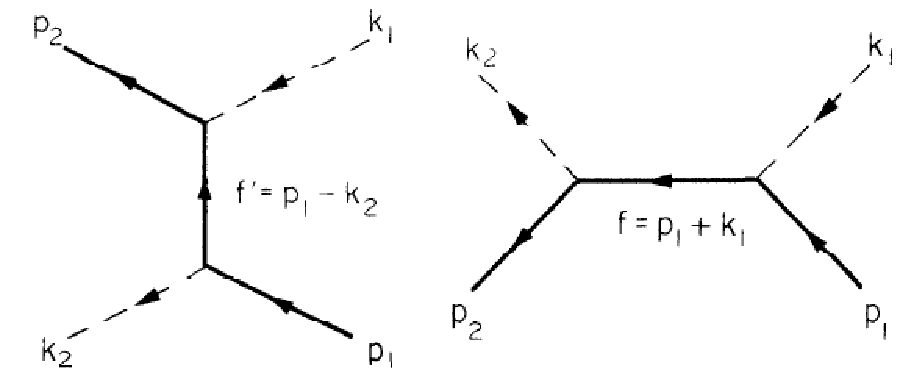
\includegraphics[width=0.7\textwidth]{Figures/Theory_of_Photon_Production_by_Inverse_Compton_Scattering/Berestetskii_ICS_Feynman.pdf}
    \caption{Two tree-level Feynman diagrams, which contributing to the matrix element of the (inverse) Compton scattering process. Left: The scattered photon is emitted with the annihilation of the incident photon, and the incident photon is absorbed with the production of the recoiling electron. Right: The incident photon and electron are absorbed, and the scattered photon is emitted with the recoiling electron. \cite{berestetskii1982quantum}}
    \label{fig:ICS_Feynman_diagrams}
\end{figure}

The general form of the electron - photon interactions can therefore be specified by
\begin{equation}
p_{1} + k_{1} = p_{2} + k_{2},
\label{eq:ICS_process}
\end{equation}

where $p_{1}$ is the four-momenta of the incident electron, $k_{1}$ is the four-momenta of the incident photon, $p_{2}$ is the four-momenta of the recoiling electron, and $k_{2}$ is the four-momenta of the scattered photon. The geometry of the inverse Compton scattering interaction in a 2D plane is shown in Fig.~\ref{fig:scattered_photon_kinematics}.

\begin{figure}[!htb]
    \centering
    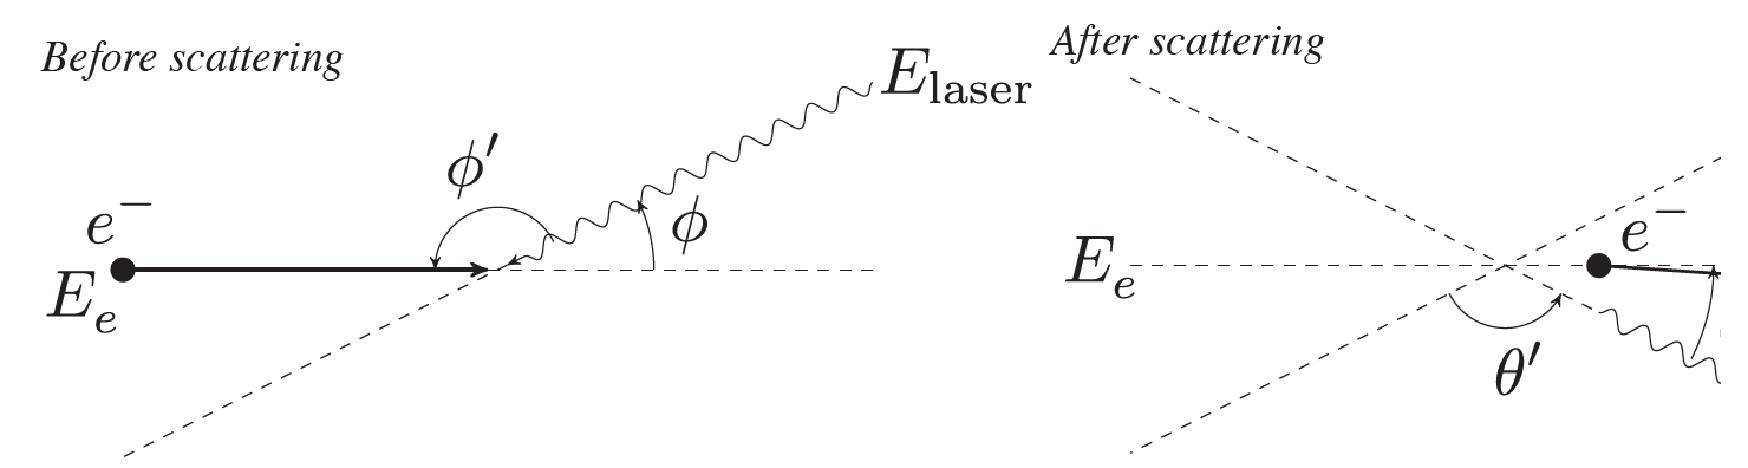
\includegraphics[width=\textwidth]{Figures/Theory_of_Photon_Production_by_Inverse_Compton_Scattering/scatteringkinematicsdiagram.pdf}
    \caption{Geometry of the inverse Compton scattering event at the interaction point. This geometry follows the geometry prescribed by Sun et al \cite{sun2009energy}. Here $\theta$ is the scattering angle of the photon, with $\phi' = \pi -\phi$ the angle between the incident electron and incident photon, where $\phi$ is the crossing angle of the electron and photon and $\theta' = \pi - \theta - \phi$ the angle between the incident and scattered photon. }
    \label{fig:scattered_photon_kinematics}
\end{figure}

\textcolor{blue}{**4-MOMENTA EQUATIONS**}

Motivated by the geometry of the inverse Compton scattering process as shown in Fig. \ref{fig:scattered_photon_kinematics}, we can write the initial photon $p_{1}$ and electron $k_{1}$ four-momenta
\begin{align}
p_{1} = \gamma m_{e}\left(c,\boldsymbol{v_{i}}\right),
\label{eq:initial_four_vectors} \\
k_{1} = \frac{E_{L}}{c}\left(1,\hat{n}_{i}\right), 
\end{align}

where $E_{L}$ is the energy of the incident photon, $\hat{n}_{i}$ is the unit displacement three-vector of the incident photon, $\gamma$ is the Lorentz factor, $m_{e}$ is the mass of the electron, $c$ the speed of light in a vacuum and $\boldsymbol{v_{i}}$ is the velocity three-vector of the incident electron with magnitude $v_{i}$. Similarly, we can present the final electron and scattered photon states with four-momenta 
\begin{align}
p_{2} = \gamma' m_{e}\left(c,\boldsymbol{v_{f}}\right), \\
k_{2} = \frac{E_{\gamma}}{c}\left(1,\hat{n}_{f}\right), 
\label{eq:final_four_vectors} 
\end{align}

where $E_{\gamma}$ is the scattered photon energy, $\hat{n}_{f}$ is the unit displacement three-vector of the scattered photon, $\gamma'$ is the Lorentz factor of the recoiling electron and $\boldsymbol{v_{f}}$ is the velocity three-vector of the recoiling electron with magnitude $v_{f}$.

\textcolor{blue}{**DERIVATION OF MANDELSTAM VARIABLES + LORENTZ INVARIANTS }

Using our four-momenta definitions (Eq.~\ref{eq:initial_four_vectors}-\ref{eq:final_four_vectors}), a  series of kinematic invariants (Mandelstam variables \cite{mandelstam1958determination}) can be determined for the photon-electron scattering process \cite{berestetskii1982quantum}
\begin{align}
s = \left(p_{1}+k_{1}\right)^{2} = \left(p_{2}+k_{2}\right)^{2},
\label{eq:s_Mandelstam} \\
t = \left(p_{1}-p_{2}\right)^{2} = \left(k_{2}-k_{1}\right)^{2},
\label{eq:t_Mandelstam} \\
u = \left(p_{1}-k_{2}\right)^{2} = \left(p_{2}-k_{1}\right)^{2}.
\label{eq:u_Mandelstam}
\end{align}

The kinematic invariants can be used to form more convenient Lorentz invariants
\begin{align}
X = \frac{s-\left(m_{e}c\right)^{2}}{\left(m_{e}c\right)^{2}},
\label{eq:X_Mandelstam} \\
Y = \frac{\left(m_{e}c\right)^{2}-u}{\left(m_{e}c\right)^{2}},
\label{eq:Y_Mandelstam}
\end{align}
which, when transformed into the geometry as shown in Fig.~\ref{fig:scattered_photon_kinematics}, can be re-wrote as
\begin{align}
X = \frac{2\gamma E_{L}\left(1-\beta\cos\phi'\right)}{m_{e}c^{2}},
\label{eq:X_geometry} \\
Y = \frac{2\gamma E_{\gamma}\left(1-\beta\cos\theta\right)}{m_{e}c^{2}},
\label{eq:Y_geometry}
\end{align}
where $\beta = v/c$, the Lorentz speed factor.

\textcolor{blue}{Do I show the full derivation of the Madelstam variables? I have done this but still...}
\textcolor{blue}{**STATEMENT OF RECOIL REGIME}

If we take the head-on case ($\phi = 0$) and  assume the incident electron is ultra-relativistic ($\beta \rightarrow 1$) then the $X$ simplifies to 
\begin{equation}
X = \frac{4\gamma E_{L}}{m_{e}c^{2}}.
\label{eq:X_headon}
\end{equation}

The Lorentz invariant $X$ can also be termed the recoil parameter, which denotes the magnitude of the recoil of the incident electron. For the case $X \ll 1$, the recoil is small and inverse Compton scattering reduces to Thomson scattering.    

\section{Non-linear Inverse Compton Scattering}

\section{Derivation of the Scattered Photon Energy Due to Inverse Compton Scattering}

\textcolor{blue}{**DERIVATION OF THE ICS SCATTERED PHOTON ENERGY**}

The relation in (Eq.~\ref{eq:ICS_process}) can be modified in order to calculate the scattered photon energy of an electron - photon interaction. Using the four-momenta in (Eq.~\ref{eq:initial_four_vectors}-\ref{eq:final_four_vectors}) we can create Lorentz invariant quantities from the Minkowski norms of the four-momenta 
\begin{align}
p_{1\mu}p_{1}^{\mu} = \gamma^{2}m_{e}^{2}\left(v^{2}-c^{2}\right) = -m_{e}^{2}c^{2},
\label{eq:lorentz_invariants1} \\
k_{1\mu}k_{1}^{\mu} = 0.
\label{eq:lorentz_invariants2}
\end{align}

We can multiply (Eq.~\ref{eq:ICS_process}) by the four-momentum  of the scattered photon and apply (Eq.~\ref{eq:lorentz_invariants2}) the Lorentz invariant 
\begin{align}
k_{2}^{\mu}\left(p_{1\mu} + k_{1\mu}\right) = k_{2}^{\mu}\left(p_{2\mu} + k_{2\mu}\right), \\
k_{2}^{\mu}p_{1\mu}+k_{2}^{\mu}k_{1\mu} = k_{2}^{\mu}p_{2\mu}.
\label{eq:apply_photon_pfinal}
\end{align}

Similarly we can construct another equation by inspecting the square of the conservation of four-momentum
\begin{align}
\left(p_{1}+k_{1}\right)_{\mu}\left(p_{1}+k_{1}\right)^{\mu} = \left(p_{2}+k_{2}\right)_{\mu}\left(p_{2}+k_{2}\right)^{\mu}, \\
p_{1\mu}p_{1}^{\mu}+k_{1\mu}p_{1}^{\mu}+k_{1\mu}p_{1}^{\mu}+k_{1\mu}k_{1}^{\mu} = p_{2\mu}p_{2}^{\mu}+k_{2\mu}p_{2}^{\mu}+p_{2\mu}k_{2}^{\mu}+k_{2\mu}k_{2}^{\mu},
\label{eq:apply_conservation_squared}
\end{align}
utilising the commutation of four-vectors ($p_{\mu}k^{\mu} = k_{\mu}p^{\mu}$) and our Lorentz invariants (Eq.~\ref{eq:lorentz_invariants1}, \ref{eq:lorentz_invariants2}) we can simplify this further 
\begin{equation}
p_{1\mu}k_{1}^{\mu} = p_{2\mu}k_{2}^{\mu}.
\label{eq:end_conservation_squared}
\end{equation}
Subbing (Eq.~\ref{eq:end_conservation_squared}) into (Eq.~\ref{eq:apply_photon_pfinal}) yields
\begin{equation}
k_{2}^{\mu}p_{1\mu}+k_{2}^{\mu}k_{1\mu} = k_{1}^{\mu}p_{1\mu}
\label{eq:substitution_four_vector}
\end{equation}

Which in three-vector notation is shown as
\begin{equation}
\frac{E_{L}E_{\gamma}}{c^{2}}\left(\hat{n}_{i}\cdot\hat{n}_{f}-1\right)+\frac{E_{\gamma}}{c}\gamma m_{e}\left(\hat{n}_{f}\cdot \boldsymbol{v_{i}}-c\right) = \frac{E_{L}}{c}\gamma m_{e}\left(\hat{n}_{i}\cdot \boldsymbol{v_{i}} -c\right)
\label{eq:three_vector_solution}
\end{equation}

However, (Eq.~\ref{eq:three_vector_solution}) should be presented in terms of the angles in Fig.~\ref{fig:scattered_photon_kinematics}. The dot products within this formula can be replaced using projections to introduce the angular dependencies
\begin{align}
\hat{n}_{i}\cdot\hat{n}_{f} = \cos\theta',
\label{eq:projection_angle_incident_scattered_photon}\\
\hat{n}_{f}\cdot \boldsymbol{v_{i}} = v_{i}\cos\theta,
\label{eq:projection_scattering_angle}\\
\hat{n}_{i}\cdot \boldsymbol{v_{i}} = v_{i}\cos\phi'.
\label{eq:projection_pi_minus_crossing_angle}
\end{align}

Upon introducing the projections (Eq.~\ref{eq:projection_angle_incident_scattered_photon}, \ref{eq:projection_scattering_angle}, \ref{eq:projection_pi_minus_crossing_angle}), (Eq.~\ref{eq:three_vector_solution}) becomes
\begin{equation}
E_{L}E_{\gamma}\left(\cos\theta'-1\right)+E_{\gamma}\gamma m_{e}c^{2}\left(\frac{v_{i}}{c}\cos\theta-1\right) = E_{L}\gamma m_{e}c^{2}\left( \frac{v_{i}}{c}\cos\phi'-1\right)
\label{eq:three_vector_solution_projections}
\end{equation}
Using the Lorentz speed factor $\beta = v/c$ and the total electron beam energy $E_{e} = \gamma m_{e}c^{2}$ and rearranging we arive at the general linear, recoil-corrected form for the scattered photon energy resulting from inverse Compton scattering 
\begin{equation}
E_{\gamma} = \frac{\left(1-\beta\cos\phi'\right)E_{L}}{1-\beta\cos\theta+\left(1-\cos\theta'\right)\frac{E_{L}}{E_{e}}}. 
\label{eq:scattered_photon_energy}
\end{equation}
  
In the head-on case, for $\theta \ll 1$ i.e. in the small angle approximation and an ultra-relativistic electron beam ($\beta \rightarrow 0$)

\begin{equation}
E_{\gamma} \approx \frac{4\gamma^{2}E_{L}}{1+\gamma^{2}\theta^{2}+X},    
\label{eq:small_angle_scattered_photon_energy}
\end{equation}
where the recoil term $X$ is given by (Eq.~\ref{eq:X_headon}). Extending this to backscattering of the incident photon ($\theta = 0$), the scattered photon energy becomes

\begin{equation}
E_{\gamma} = \frac{4\gamma^{2}E_{L}}{1+X},
\label{eq:headon_backscattering_scattered_photon_energy}
\end{equation}
which is referred to in the literature \cite{krafft2010compton} as the Compton edge. The $\gamma^{2}$ factor within this equation refers to the double Doppler shift experienced by the incident photon as it is scattered.

\section{Electron - Photon Interaction Cross Section}

\textcolor{blue}{**THE CROSS SECTION FORMULA** \\ \textit{Where does this need to go, need to fix an order.}}

The cross section for the inverse Compton scattering interaction \cite{landau1982course} is given by \textcolor{blue}{is this excluding non-linear effects?}

\begin{equation}
 \sigma_{c} = \frac{2\pi r_{e}^{2}}{X}\left[\frac{1}{2}+\frac{8}{X}-\frac{1}{2\left(1+X\right)^{2}}+\left(1-\frac{4}{X}-\frac{8}{X^{2}}\right)\log{\left(1+X\right)}\right],
 \label{eq:compton_cross_section}
\end{equation}
where $r_{e}$ is the classical radius of the electron. If we take the limit of this in the classical limit ($X \to 0$) we obtain

\begin{equation}
\lim_{X \to 0} \sigma_{c} = \frac{8\pi r_{e}^{2}}{3}\left(1-X\right) = \sigma_{T}\left(1-X\right),
\label{eq:compton_cross_section_classical_limit}
\end{equation}
where $\sigma_{T}$ is the Thomson cross section. Where the interaction is firmly in the classical regime ($X \ll 1$), in which inverse Compton scattering becomes Thomson scattering and there is elastic scattering, the Compton cross section recovers the Thomson scattering cross section, $\sigma_{c} = \sigma_{T}$. If we take the ultra-relativistic limit ($X \to \infty$) of the cross section, the cross section becomes

\begin{equation}
\lim_{X \to \infty} \sigma_{c} = \frac{2\pi r_{e}^{2}}{X}\left(\log{X}+\frac{1}{2}\right).
\label{eq:compton_cross_section_ultrarelativistic_limit}
\end{equation}

\textcolor{blue}{**WOULD IT BE WORTHWHILE HAVING A GRAPH HERE TO SHOW CROSS SECTION VS ENERGY**}

Following the derevation by Berestetskii et al \cite{landau1982course} and using the notation of Sun and Wu \cite{sun2011theoretical}, the inverse Compton scattering cross section is given by

\begin{equation}
\frac{d\sigma}{d\Omega} = \frac{8r_{e}^{2}}{X^{2}}\left\{\left[1+P_{t}\left(2\tau-2\phi_{f}\right)\right]\left[\left(\frac{1}{X}-\frac{1}{Y}\right)^{2}+\frac{1}{X}+\frac{1}{Y}\right]+\frac{1}{4}\left(\frac{X}{Y}+\frac{Y}{X}\right)\right\}\left(\frac{E_{\gamma}}{mc^{2}}\right)^{2},    
\end{equation}
where $d\Omega = \sin\theta d\theta d\phi_{f}$ is the differential solid angle, $P_{t}$ is the degree of linear polarisation, $\tau$ is the azimuthal angle of the linear polarization with respect to the $x$ axis, $\phi_{f}$ is the azimuthal angle of the scattering plane and the Lorentx invariant quatity $Y$ is given by

\begin{equation}
Y = \frac{2\gamma E_{\gamma}\left(1-\beta\cos\theta\right)}{mc^{2}}.
\label{eq:cross_section_Y}    
\end{equation}

For a circular or unpolarised incident laser this is negligible ($P_{t}=0$), however this is non-zero for linear polarised cases ($P_{t}\neq0$). Therefore, the distribution of scattered photons is azimuthally symetric for the circularly or unpolarized case polarised case but azimuthally modulated and asymmetric for the linear polarisation case \cite{sun2011theoretical}.  

\section{Luminosity and Flux}
\textcolor{blue}{**DERIVATION FROM LARMOR THEOREM TO HEAD-ON LUMINOSITY**}
Using Larmor's theorem \textcolor{blue}{[citation please!]} and following the the derivation by Krafft and Priebe \cite{krafft2010compton} the luminosity of an ICS source in the head on case can be derived. \textcolor{blue}{text needs work}

Larmor's theorem
\begin{equation}
P_{rad} = \frac{\gamma^{4}e^{2}}{6\pi \epsilon_{0}c^{3}}\lvert\mathbf{\dot{v}}\rvert^{2} = \gamma\sigma_{c}\epsilon_{0}c\lvert\left(\mathbf{E}+\mathbf{v}\times\mathbf{B}\right)\mathbf{x}\left(t\right)\rvert^{2},
\label{eq:larmor_formula}    
\end{equation}
where $e$ is the charge of an electron,  $\epsilon_{0}$ is the permitivity of free space, $c$ is the speed of light in a vacuum, $\lvert\mathbf{\dot{v}}\rvert$ is the acceleration of the electron in the laboratory frame, $\sigma_{c}$ is the Klein-Nishsina cross section, $\mathbf{E}$ and $\mathbf{B}$ are respectively the electric field and magnetic flux density of the incident laser, $\lvert\mathbf{v}\rvert$ is the velocity of the electron as it traverses the laser pulse and $\mathbf{x}\left(t\right)$ is the first order approximation of the orbit of the electron as it traverses the incident laser pulse. 

The total energy radiated by the electron $U_{e^{-}}$ is given by

\begin{equation}
U_{e^{-}} = \int P\left(t\right)dt = \gamma^{2}\left(1+\beta\right)^{2}\sigma_{c}\epsilon_{0}\int\lvert\mathbf{E}\left(x,y,z\right)\rvert^{2}dz,
\label{eq:electron_radiated_energy}
\end{equation}

If we take the head-on case ($\phi=0$) where the electron bunch and the laser pulse can be represented by a Gaussian intensity function and apply the plane wave approximation to the laser pulse, where the energy density of a plane wave laser is $\epsilon_{0}\lvert\mathbf{E}\rvert^{2}$, the total energy of the scattered photons $U_{\gamma}$ becomes

\begin{equation}
U_{\gamma} = \gamma^{2}\left(1+\beta\right)\sigma_{c}\frac{N_{e}N_{L}}{2\pi\sqrt{\sigma_{x,e}^{2}+\sigma_{x,L}^2}\sqrt{\sigma_{y,e}^{2}+\sigma_{y,L}^{2}}}\hbar\omega,
\label{eq:total_interaction_energy}
\end{equation}
where $N_{e}$ is the number of electrons in the interacted bunch, $N_{L}$ is the number of photons in the laser pulse, $\sigma_{x/y,e}$ is the transverse \textit{rms} radius of the electron bunch at the IP and $\sigma_{x/y,L}$ is the transverse \textit{rms} radius of the laser pulse spot at the IP in either the $x$ or $y$ plane. This formula also omits the hourglass effect of the two diverging beams.

Using the average scattered photon energy $\gamma^{2}\left(1+\beta\right)\hbar\omega$ \textcolor{blue}{should prove this elsewhere} we can convert this to $N_{\gamma}$, the number of photons produced from a single electron bunch - laser pulse interaction

\begin{equation}
N_{\gamma} = \sigma_{c}\frac{N_{e}N_{L}}{2\pi\sqrt{\sigma_{x,e}^{2}+\sigma_{x,L}^2}\sqrt{\sigma_{y,e}^{2}+\sigma_{y,L}^{2}}}.
\label{eq:no_photon_headon}
\end{equation}

The total flux of the photons is given by $\mathcal{F} = N_{\gamma}\cdot f$ where $f$ is the repetition frequency of the ICS source.

\section{Angular Crossing and Hourglass Effects}

\textcolor{blue}{**DERIVATION FOR THE ANGULAR CASE, Miyahara \cite{miyahara2008luminosity}or Suzuki \cite{suzuki1976general}**}

The flux in the case of an angular crossing is given by 

\begin{equation}
F = \sigma_{c}\frac{N_{e}N_{L}f\cos\phi}{2\pi\sigma_{y}\sqrt{\sigma_{x}^{2}\cos^{2}\phi + \sigma_{z}^{2}\sin^{2}\phi}},
\label{eq:crossing_angle_flux}
\end{equation}
where $\sigma_{i}(i=x,y,z) = \sqrt{\sigma_{i,e}^{2}+\sigma_{i,L}^{2}}$ with $\sigma_{z,e}$ the electron \textit{rms} bunch length and $\sigma_{z,L}$ the laser \textit{rms} pulse length.

\textcolor{blue}{**DERIVATION FOR THE HOURGLASS EFFECT**}

\section{Collimated Flux + Investigation}

\section{Spectral Density}

\section{Peak and Average Brilliance}
\textcolor{blue}{**DERIVATION OF THE AVERAGE BRILLIANCE \\ Is this necessary?? Is it enough to say flux per area in phase space?}

The average brilliance is defined as the flux per unit phase space area of the interaction per 0.1\% bandwidth and is subsequently given by \cite{krafft2010compton,deitrick2018high} \textcolor{blue}{is this the correct source, did they get it from somewhere else earlier?}

\begin{equation}
B_{\mathrm{avg}} = \frac{\mathcal{F}_{0.1\%}}{4\pi^{2}\sigma_{\gamma,x}\sigma_{\gamma,x'}\sigma_{\gamma,y}\sigma_{\gamma,y'}},
\label{eq:average_brightness}
\end{equation}
where $\mathcal{F}_{0.1\%}$ is the flux in a 0.1\% bandwidth, $\sigma_{\gamma,x/y}$ are the source sizes in each plane and $\sigma_{\gamma,x'/y'}$ are the angular divergences in each plane.


\section{Bandwidth + Investigation}

The bandwidth, the energy spread of the scattered photons, is given in the recoil corrected non-linear regime ($a_{0}\ll 1$) \cite{ranjan2018simulation} by

\begin{equation}
\frac{\Delta E_{\gamma}}{E_{\gamma}} = \sqrt{\left(\frac{\sigma_{\theta}}{E_{\theta}}\right)^{2}+\left(\frac{\sigma_{e}}{E_{e}}\right)^{2}+\left(\frac{\sigma_{L}}{E_{L}}\right)^{2}+\left(\frac{\sigma_{\epsilon}}{E_{\epsilon}}\right)^{2}},
\label{eq:bandwidth}    
\end{equation}
where $\frac{\sigma_{\theta}}{E_{\theta}}$ is the collimation term, $\frac{\sigma_{e}}{E_{e}}$ is the electron beam energy spread term, $\frac{\sigma_{L}}{E_{L}}$ is the laser pulse energy spread term and $\frac{\sigma_{\epsilon}}{E_{\epsilon}}$ is the emittance terms. These terms are given by

\begin{equation}
\frac{\sigma_{\theta}}{E_{\theta}} = \frac{1}{\sqrt{12}}\frac{\psi^{2}}{1+X+\psi^{2}/2}
\label{eq:collimation_term}
\end{equation}

\begin{equation}
\frac{\sigma_{e}}{E_{e}} = \frac{2+X}{1+X+\psi^{2}}
\label{eq:beam_energy_spread_term}
\end{equation}

\begin{equation}
\frac{\sigma_{L}}{E_{L}} = \frac{1+\psi^{2}}{1+X+\psi^{2}}
\label{eq:laser_energy_spread_term}
\end{equation}

\begin{equation}
\frac{\sigma_{\epsilon}}{E_{\epsilon}} = \frac{\sqrt{2}\gamma^{2}}{1+X}\sqrt{\frac{\epsilon_{x}^{2}}{\beta_{x}^{*2}}+\frac{\epsilon_{y}^{2}}{\beta_{y}^{*2}}}    
\end{equation}
where $\psi = \gamma\theta$ is the acceptance angle, $\epsilon_{x/y}$ is the emittance in the $x$ or $y$ direction and $\beta_{x/y}^{*}$ are the $\beta$ functions at the IP in both directions.



\end{document}